\documentclass{article}
\usepackage{geometry}
\geometry{legalpaper,  margin=0.5in}
\usepackage[utf8]{inputenc}
\usepackage{amsmath}
\usepackage{amssymb}
\usepackage{amsfonts}
\usepackage{graphicx}
\usepackage{subcaption}

\usepackage[dvipsnames]{xcolor}
\newcommand{\todo}{\textcolor{blue}{TODO} : }
\newcommand{\done}{\textcolor{LimeGreen}{DONE} : }
\newcommand{\doing}{\textcolor{Purple}{DOING} : }
\newcommand{\issue}{\textcolor{red}{ISSUE} : }
\newcommand{\pending}{\textcolor{RedOrange}{PENDING} : }

\title{Report on Hyperpolic Community detection}
\author{}
\begin{document}
    \maketitle
    \section{Introduction}

        We plan to adapt the paper "Learning Community Embedding with Community Detection and Node Embedding on Graphs"
        using Hyperbolic space instead of euclidean one.
        Today community graph embedding rely on projecting data from a graph (such as adjacency matrix) on an continuous 
        space, and the retrieve community by clustering based algorithms.
        The  projection often involve a small representation space, moreover severall communauties are overlapping each others.
        In particular hierarchical community can exists, taking it into account can be relevant.
        If mainly used representation space is euclidean, some others manifolds can be used.
        Particularly hyperbolic manifolds have prooven their efficiency to embed hierarchical data and performs well in low dimenssion space.
        In this document we report results and experiments in progress experiments on community detection using hyperbolic riemnanian manifolds.

    \section{Learning Community Embedding with Community Detection an Node Embedding Graph}
    Before describing our approach we sum up the main related articles.  The paper propose to face Community detection in jointly learning detection process and embedding projection function.

    \subsection{Community Detection embedding}
        In order to retrieve community, authors propose to associate for each examples embeddings a community probability by $p(z_i=k)$ the probability of node $v_i$ to belong to the community indexed by $k$. They model the prosteriot $p(v_i|z, \Theta)$ by a multivariate gaussian distritbution, thus we can write :
        $$
            p(v_i |z_i = k; \phi_i, \psi_k, \Sigma_k) = \mathcal{N}(\phi_i| \psi_k, \Sigma_k)
        $$
        With $\psi_k$, $\Sigma_k$ respectively the mean and variance of the gaussian distribution.

    \subsection{Node Embedding}
        The embeddings are obtained by rapproaching neigbhors in terms of graph distance, the first cost function associate is : 
         $$
            O_1 = -\alpha_1 \sum \limits_{(v_i, v_j) \in E} log(\sigma(z_i^tz_j)))
         $$
         with $E$ the vertices.
         Unfortunatelly nodes at distance one are not always in the same community and nodes at a further distance can be in a same community.
         Thus the \textit{DeepWalk} algorithm propose to perform a random walk over the graph allowing to find neigbhors. 
         The neigbhorhood of a node $v_i$ is called context of $v_i$, denoted $C_i$:

        $$
            O_2 = -\alpha_2  \sum \limits_{v_i\in V} \sum \limits_{v_j \in C_i} \bigg[  log(\sigma(z_i^tz_j))) + \sum \limits_{t=1, v_l \notin C_i}^T log(\sigma(z_i^t z_l)) \bigg]
        $$
        Once the model is fit we must ensure that it fit the multivariate gaussian prior.
        To connect both, the node embedding must take into account detection process, thus they add an additional loss fixing all except the embedding.
        This is given by :
        $$
            O_3 = - \alpha_3 \sum\limits_{v_i \in V} log\bigg[\sum\limits_{k=1}^K p(z_i=k)p(v_i|z_i=k;\phi_i,\psi_k,\Sigma_k)\bigg]
        $$

    \section{Adapting to Hyperbolic}
        \subsection{Node Embedding without a priori on Community detection}
            In this section we plan to find an alternative to $O_1$ and $O_2$ loss function because we can not use $O_1$ and $O_2$ without considering the poincaré ball distance.
            To keep the same meaning we can modelize the propabilities of users being in the same community  $P((v_i,v_j)\in C | z_i, z_j)$ we can thus simply modelise it by an exponential distribution :
            $$
            p((v_i,v_j)\in E | z_i, z_j) = \lambda e^{-\lambda -d_h(z_i,z_j)}
            $$
            with $d_h$ the distance associate to the hyperbolic space.
            Thus we can use the following loss function considering that items sharing edge often are in the same community :
            $$
                O_{h,1} =  - \alpha_1 \sum_{(v_i,v_j) \in E} log(p((v_i,v_j)\in C | z_i, z_j) )
            $$
            With $\lambda$ a parameter that may be selected by grid search, however we curently use in experiments $\lambda=1$.



            \paragraph{}
            We also need to adapt a loss using negative sampling and randomWalks
            \begin{align*}
                O_{h,2} &= - \alpha_2 \sum_{(v_i,v_j)\in R} log\Bigg[ \frac{p((v_i,v_j)\in C | z_i, z_j)}{\sum\limits_{v_k \in N_i \cup v_j}p((v_i,v_k)\in E | z_i, z_k)}\Bigg] \\
                  & = \alpha_2 \sum_{(v_i,v_j)\in R} log \Bigg[1 + \sum\limits_{v_k \in N_i \cup v_j} \lambda e^{-\lambda(d_h(z_i,z_j) - d_h(z_i,z_k))} \Bigg]
            \end{align*}

            For optimization we use gradient descent with retractation similarly to the Nickel et al paper \cite{poincareWTV}.
            We may also use the gradient descent proposed by Wilson and Leimeister \cite{PoincareGradient}, showing better convergence on severall tasks, similarly we can also use the lorentz model method Kiala et al \cite{LorentzEmbeddings} and then projecting in the poincaré model.

            Considering $f_\theta: x \rightarrow r $ the projection function and $L(x,y)$ the loss function, the Nickel et al methods update the parameters $\theta$ by :
            $$
                \theta_{t+1} = \theta_{t} - \alpha \frac{(1- ||\theta_t||^2)^2 }{4}\Delta_E
            $$

            With $\Delta_E$ the gradient of loss function with respect to $\theta_t$

            The second method proposed is based on optimization on the tangent space and then using exponential map to remap gradient on the hyperbolic space. 
            \subsection{EM}

            % We can write $P(x | p, \mu) = \sum \limits_{k=0}^K p_k  \frac{1}{\zeta(i)}e^{\frac{-(d_h(x,\mu_k))^2} {2\sigma_k^2}} $.

            \subsection{Connecting both}
                
                To connect both embeddings must fit the prior,
                This is done by minimizing :
                $$
                    O_{h,3} = -\alpha_3   \sum_{v_i\in V} log\Bigg[ \pi_{ik}\sum \limits_{k=0}^K \frac{1}{\zeta(i)}e^{\frac{-(d_h(x,\mu_k))^2}{2\sigma_k^2}}\Bigg]
                $$
                $$
                    O_{h,3}' =-\alpha_3  \sum_{v_i\in V}  \sum \limits_{k=0}^K \pi_{ik} log\Bigg[\frac{1}{\zeta(i)}e^{\frac{-(d_h(x,\mu_k))^2}{2\sigma_k^2}}\Bigg]
                $$
                $$
                    O_{h,3} \leq O_{h,3}' 
                $$

    \section{Evaluating EM Algorithm On large dataset}

    \begin{figure}[!ht]
        \centering
        \begin{subfigure}[b]{0.48\linewidth}
            \centering
            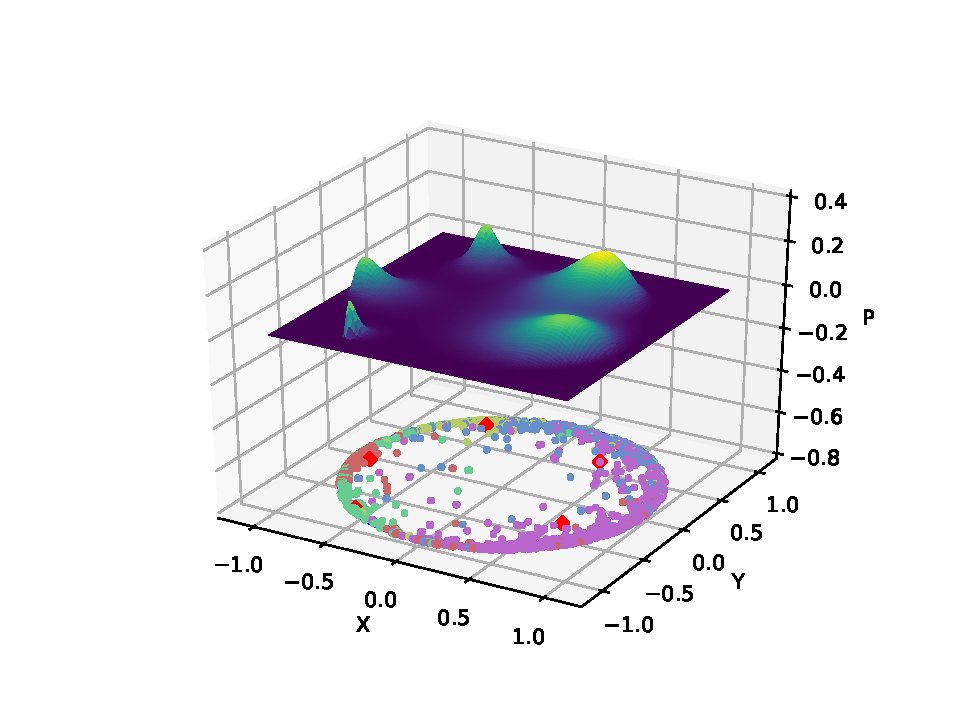
\includegraphics[scale=0.5]{media/fig0.pdf}
            \caption{\label{fig:n1}:Kmeans only}
        \end{subfigure}
        \begin{subfigure}[b]{0.48\linewidth}
             \centering
            \includegraphics[scale=0.5]{media/fig1.pdf}
            \caption{\label{fig:n2}: $1^{st}$ EM iteration}
    
        \end{subfigure}
        \begin{subfigure}[b]{0.48\linewidth}
            \centering
            \includegraphics[scale=0.5]{media/fig2.pdf}
            \caption{\label{fig:n1}:$2^{nd}$ EM iteration}
        \end{subfigure}
        \begin{subfigure}[b]{0.48\linewidth}
             \centering
            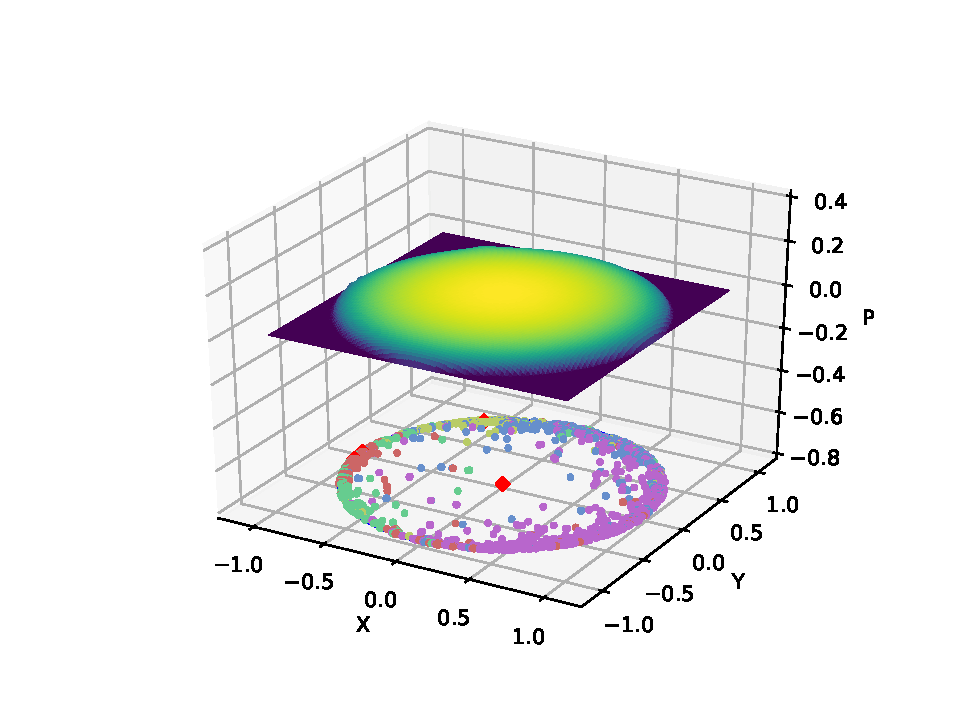
\includegraphics[scale=0.5]{media/fig50.pdf}
            \caption{\label{fig:n2}:$50^{nd}$ EM iteration}
    
        \end{subfigure}    
        \caption{EM over a dblp representation}
        \label{fig:embedding}
    \end{figure}
    \subsection{Variance and mixing coefficient evolution}

    \begin{figure}[!ht]
        \centering
        \begin{subfigure}[b]{0.48\linewidth}
            \centering
            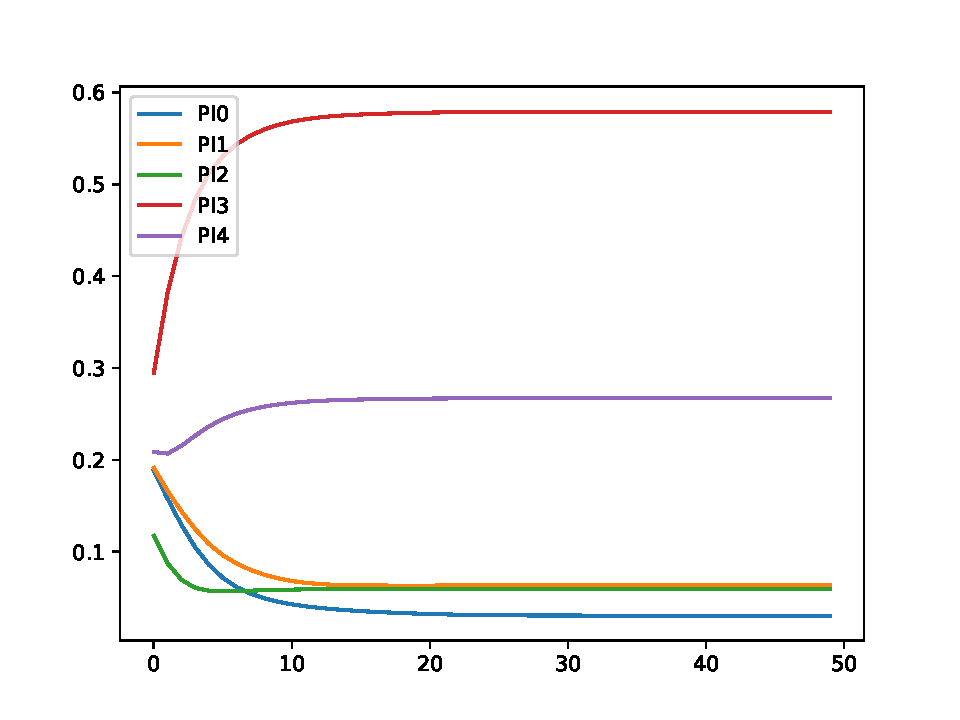
\includegraphics[scale=0.5]{media/_mixture_weights.pdf}
            \caption{\label{fig:n1}:Mixture weights}
        \end{subfigure}
        \begin{subfigure}[b]{0.48\linewidth}
             \centering
            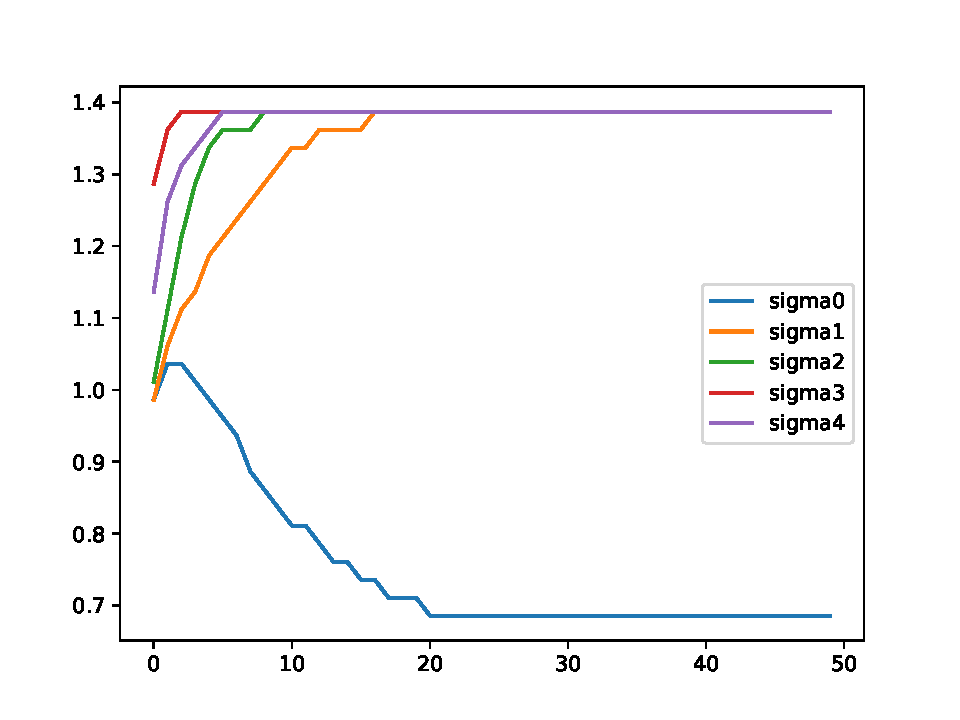
\includegraphics[scale=0.5]{media/_variances.pdf}
            \caption{\label{fig:n2}:variance}
    
        \end{subfigure}
        \caption{EM over a dblp representation}
        \label{fig:embedding}
    \end{figure}

    \section{Experiments}
    \begin{table}
            \begin{tabular}{|cccccccc|c|}
                \hline
                lr & alpha & beta & gamma & Method Optimization& epoch & embed iter &em iter & Performances \\
                \hline
                .5 & .5 & 10.& 20 & exphsgd & 3 & 600 & 1 & 78.81 \\
                \hline
            \end{tabular}
        \label{DBLP-RES}
        \caption{DBLP Performances obtained 1 Disc}
    \end{table}

    \subsection{Compareason KMEANS-EM}
    \begin{table}
        \begin{tabular}{|ccccccccc|c|}
            \hline
            lr & alpha & beta & dim & Method Optimization& epoch & embed iter &em iter & Performances & REF-FILE\\
            \hline
            10 & .1 & 1.& 2 & exphsgd & 1 & 1000 & 1 & $69.56 \pm 7.38$& football-1\\
            10 & .1 & 1.& 3 & exphsgd & 1 & 1000 & 1 & $79.13 \pm 1.23$& football-3D-1\\
            10 & .1 & 1.& 4 & exphsgd & 1 & 1000 & 1 & $84.16 \pm 3.43$& football-4D-1\\
            10 & .1 & 1.& 10 & exphsgd & 1 & 1000 & 1 & $87.38 \pm 1.84$& football-10D-1\\
            \hline
        \end{tabular}
    \label{DBLP-RES}
    \caption{FOOTBALL Performances obtained  with kmeans (2 experiments each)}
\end{table}
    \begin{table}
        \begin{tabular}{|ccccccccc|c|}
            \hline
            lr & alpha & beta & dim & Method Optimization& epoch & embed iter &em iter & Performances & REF-FILE\\
            \hline
            10 & .1 & 1.& 2 & exphsgd & 1 & 1000 & 1 & $76.08 \pm 0.615$& football-1D-1EM\\
            10 & .1 & 1.& 3 & exphsgd & 1 & 1000 & 10 & $86.08 \pm 1.23$& football-3D-1-EM\\
            10 & .1 & 1.& 4 & exphsgd & 1 & 1000 & 10 & $87.82 \pm 1.23$& football-4D-1-EM\\
            10 & .1 & 1.& 10 & exphsgd & 1 & 1000 & 10 & $91.3 \pm 0$& football-10D-1-EM\\
            \hline
        \end{tabular}
    \label{DBLP-RES}
    \caption{FOOTBALL Performances obtained  with EM (2 experiments each)}
\end{table}
\begin{table}
    \begin{tabular}{|ccccccccc|c|}
        \hline
        lr & alpha & beta & dim & Method Optimization& epoch & embed iter & context & Performances & REF-FILE\\
        \hline
        1.0 & .1 & 1.& 2 & exphsgd & 1 & 1000 & 17 & LAUNCHED& \\

        \hline
    \end{tabular}
\label{DBLP-RES}
\caption{DBLP Performances KEMANS (2 experiments each)}
\end{table}
\begin{table}
    \begin{tabular}{|ccccccccc|c|}
        \hline
        lr & alpha & beta & dim & Method Optimization& epoch & embed iter & context & Performances & REF-FILE\\
        \hline
        20 & .1 & 1.& 2 & exphsgd & 1 & 500 & 17 & $69.49 \pm 6.78$& DBLP-2D-KMEANS \\
        20 & .1 & 1.& 3 & exphsgd & 1 & 500 & 17 & RUNNING& DBLP-2D-KMEANS \\
        20 & .1 & 1.& 4 & exphsgd & 1 & 500 & 17 & $80.8 \pm 1.42$& DBLP-4D-KMEANS \\
        20 & .1 & 1.& 10 & exphsgd & 1 & 500 & 17 & RUNNING & DBLP-2D-KMEANS \\

        \hline
    \end{tabular}
\label{DBLP-RES}
\caption{DBLP Performances KEMANS (2 experiments each)}
\end{table}
\begin{figure}[!ht]
    \centering

        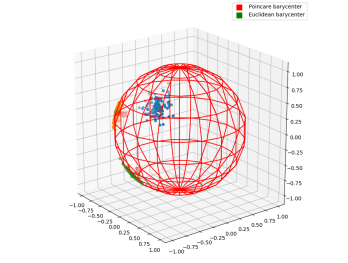
\includegraphics[scale=2]{media/kmeans3d.png}
        \caption{3D kmeans}

\end{figure}

\end{document}